
\section{Распознавание вторжений в БД}



\subsection{Основные понятия}

\textbf{Вторжение в БД} -- незаконное или несанкционированное проникновение в базу данных с целью получения несанкционированного доступа к конфиденциальной информации или изменения данных.

\textbf{Обнаружение вторжений} (применительно к БД) -- процесс выявления действий,
которые способны нарушить конфиденциальность, целостность и доступность информации,
хранимой в БД.

\textbf{Система обнаружения вторжений (СОВ)} (англ. Intrusion Detection System / IDS / ID-system) -- программное или программно-техническое средство, предназначенное для автоматизированного обнаружения несанкционированных и вредоносных действий в информационной системе, а также оповещения ИБ-специалистов об обнаруженных нарушениях \cite{kasperskyIDS}.

СОВ не обладают функциями реагирования (напр., блокировки) на нежелательную активность, поэтому применение СОВ относится к реактивным мерам (то есть к таким мерам, которые используются уже после того, как произошел инцидент) для противодействия активности злоумышленника в тех случаях, когда злоумышленник преодолел все проактивные меры. Обычно системы обнаружения вторжений используются в качестве \textit{вторичного фактора защиты в общей системе защиты}.



\subsection{Предотвращение вторжений в БД}

\textbf{Система предотвращения вторжений} (англ. Intrusion Prevention Sysytem / IPS) -- программное или программно-техническое средство, предназначенное для обнаружения и пресечения несанкционированных и вредоносных действий в информационной системе. В отличие от IDS, IPS может не только уведомлять ИБ-специалистов о факте нарушения, но и самостоятельно противодействовать атакам, напр., блокируя соединение или настраивая межсетевой экран \cite{kasperskyIPS}.

Системы предотвращения вторжений являются расширением систем обнаружения вторжений, так как IPS системы так же как и IDS должны обладать возможностью обнаружения вторжений. Иначе говоря, IPS системы являются активными IDS системами.

Архитектура IDS включает:
\begin{itemize}
	\item сенсорную подсистему, предназначенную для сбора событий, связанных с безопасностью защищаемой системы
	
	\item подсистему анализа, предназначенную для выявления атак и подозрительных действий на основе данных сенсоров
	
	\item хранилище, обеспечивающее накопление первичных событий и результатов анализа
	
	\item консоль управления, позволяющая конфигурировать IDS, наблюдать за состоянием защищаемой системы и IDS, просматривать выявленные подсистемой анализа инциденты
\end{itemize}

Архитектура IPS включает в себя все компоненты IDS, а также:
\begin{itemize}
	\item подистему реагирования, принимающую решение о способе противодействия выявленным атакам
\end{itemize}

\textit{(Здесь и далее будет использоваться преимущественно термин СОВ/IDS, но нужно понимать, что все функции и особенности IDS также распространяются и на IPS)}

\subsubsection{Типы моделей систем распознавания вторжений (ID-систем)}

Существует множество способов классификации СОВ, которые не являются однозначными или
обязательными. Следует рассмотреть наиболее известные и используемые классификации,
которые характеризуют систему по:
\begin{itemize}
	\item \textbf{По способу мониторинга}

	\item \textbf{По способу анализа}

	\item \textbf{По скорости реакции}

	\item \textbf{По классу защиты}
\end{itemize}

\paragraph*{По способу мониторинга \cite{kasperskyIDS}.}

\begin{itemize}
	\item \textbf{Сетевая СОВ (англ. Network-based IDS, NIDS)} -- система,
	которая занимается проверкой сетевого трафика с концентратора или коммутатора и
	анализируя сетевые пакеты.

	\item \textbf{Узловая СОВ (англ. Host-based IDS, HIDS)} -- система,
	отслеживающая вторжения, используя анализ системных вызовов, логов приложений,
	модификаций файлов (исполняемых, файлов паролей, системных баз данных), состояния
	хоста и прочих источников.
	
	\item \textbf{Основанная на протоколе СОВ (англ. Protocol-based IDS, PIDS)} -- система, которая отслеживает и анализирует коммуникационные протоколы со связанными системами или пользователями. Для веб-сервера подобная СОВ обычно ведет наблюдение за HTTP и HTTPS протоколами. При использовании HTTPS СОВ должна располагаться на таком интерфейсе, чтобы просматривать HTTPS пакеты ещё до их шифрования и отправки в сеть.

	\item \textbf{Основанная на прикладных протоколах СОВ (англ. Application-based IDS, APIDS)} --
	система, в которой ведется наблюдение за специализированными прикладными протоколами
	и анализ соответствующих данных. Например, на веб-сервере с SQL базой данных СОВ будет
	отслеживать содержимое SQL команд, передаваемых на сервер.

	\item \textbf{Гибридная СОВ} -- система, которая является композицией нескольких видов
	систем обнаружения вторжений.
\end{itemize}


\paragraph*{По способу анализа.}

Данная классификация строится по способу анализа событий, полученных из источника информации, и методу принятия решения, что происходит проникновение. Согласно классификации, предложенной Стефаном Аксельсоном, выделяют три типа методов обнаружения вторжения \cite{IDSClassification}:

\textbf{на основе сигнатур} (англ. misuse detection) - это методы, которые обнаруживают вторжения путём сравнения инструкций / SQL-запросов с шаблонами недопустимых синтаксических конструкций, используемых вредоносным ПО. Термин сигнатура берет начало в антивирусном программном обеспечении, которое впервые называет эти обнаруженные шаблоны сигнатурами. Хотя IDS на основе сигнатур могут легко обнаружить известные атаки, им сложно выявить новые атаки, для которых еще не существует шаблонов \cite{NetSecChristos}.

\textbf{на основе аномалий} (англ. anomaly detection) -- это методы, которые наоборот, в отличие от первого типа, подрузамевают создание шаблонов нормального поведения пользователя и последующее сравнение этих шаблонов с действиями, выполняемыми пользователями во время работы с БД. Эти методы были созданы в первую очередь для обнаружения неизвестных атак, отчасти из-за быстрого развития вредоносного ПО. Хотя такой подход позволяет обнаруживать ранее неизвестные атаки, он может страдать от ложных срабатываний: ранее неизвестная легитимная активность может быть классифицирована как вредоносная. Также, большинство существующих IDS страдают от того, что процесс обнаружения занимает много времени, что снижает производительность. 

\textbf{на основе смешанных методов} -- представляет собой композицию первых двух методов.

\paragraph*{По скорости реакции.}

Определяют два типа СОВ по времени между получением информации из источника и ее
анализом и принятием решения. В зависимости от задержки во времени, СОВ разделятся на:
\begin{itemize}
	\item \textbf{с пакетным режимом (англ. interval-based)}. В таких системах реакция
	происходит через определенные интервалы времени, а информационный поток от точек
	мониторинга до инструментов анализа не является непрерывным.

	\item \textbf{непрерывные (англ. real-time)}. В таких системах обрабатывается
	непрерывный поток информации от источников. При этом таких тип является преобладающей
	типом в сетевых СОВ, которые получают информацию из потока сетевого трафика.
\end{itemize}


\paragraph*{По классу защиты.}

Для каждой сертифицированной в России СОВ присваивается некоторый класс защиты
согласно классификации ФСТЭК и выполненным требованиям для определенного профиля защиты (ПЗ).
Всего существует 6 классов, где самый низкий класс - шестой, а самый высокий - первый.

Согласно ФСТЭК СОВ разделяются на \cite{IDSFSTEK}:
\begin{itemize}
	\item \textbf{СОВ с 6 классом защиты}: применяются в информационных системах
	персональных данных 3 и 4 классов.

	\item \textbf{СОВ с 5 классом защиты}: применяются в информационных системах
	персональных данных 2 класса.

	\item \textbf{СОВ с 4 классом защиты}: применяются в государственных информационных
	системах, в которых обрабатывается информация ограниченного доступа, не содержащая
	сведения, составляющие государственную тайну, в информационных системах персональных
	данных 1 класса, а также в информационных системах общего пользования II класса.

	\item \textbf{СОВ с 3, 2 или 1 классом защиты}: применяются в информационных системах,
	в которых обрабатывается информация, содержащая сведения, составляющие государственную
	тайну.
\end{itemize}



\subsubsection{Общая структура ID-систем}


\paragraph*{Архитектура СОВ.} Основнымы архитектурными компонентами СОВ являются:

\begin{enumerate}
	\item \textbf{Host} -- система, на которой выполняется ПО СОВ.

	\item \textbf{Target} -- система, за которой наблюдает СОВ.
\end{enumerate}

Первоначально многие СОВ выполнялись на тех же системах, которые они защищали.
Основная причина этого была в том, что большинство систем было mainframe, и стоимость
выполнения СОВ на отдельном компьютере была очень большой. Это создавало проблему с
точки зрения безопасности, так как любой атакующий, который успешно атаковал целевую
систему, мог в качестве одной из компонент атаки просто запретить функционирование СОВ.

Но с появлением рабочих станций и персональных компьютеров в большинстве архитектур
СОВ предполагается выполнение СОВ на отдельной системе, тем самым разделяя системы
Host и Target. Это улучшает безопасность функционирования СОВ, так как в этом случае
проще спрятать существование СОВ от атакующих.

\paragraph*{Способы управления СОВ:}

\begin{itemize}
	\item \textbf{Централизованное управление}. При централизованных стратегиях управления
	весь мониторинг, обнаружение и отчетность управляются непосредственно с единого "поста".
	В этом случае существует единственная консоль СОВ, которая связана со всеми сенсорами,
	расположенными в сети.

	\item \textbf{Частично распределенное управление}. Мониторинг и определение управляются
	с локально управляемого узла, с иерархической отчетностью в одно или более центральных
	расположений.

	\item \textbf{Полностью распределенное управление}. Мониторинг и определение выполняются
	с использованием подхода, основанного на агентах, когда решения об ответе делаются в
	точке анализа.
\end{itemize}

При этом в сети должны поддерживаться следующие связи:

\begin{itemize}
	\item связи для передачи отчетов СОВ. Эти связи создаются между сенсорами как сетевого
	мониторинга, так и мониторинга хоста, и центральной консолью СОВ;

	\item связи для мониторинга хостов и сетей;

	\item связи для выполнения ответов СОВ.
\end{itemize}

\subsubsection{Определение сигнатур (злоупотреблений)}

Детекторы злоупотреблений анализируют деятельность системы, анализируя событие или множество событий на соответствие заранее определенному образцу, который описывает известную атаку. Соответствие образца известной атаке называется сигнатурой, определение злоупотребления иногда называют ``сигнатурным определением''. Наиболее общая форма определения злоупотреблений, используемая в коммерческих продуктах, специфицирует каждый образец событий, соответствующий атаке, как отдельную сигнатуру. \autocite{IntrusionDetectionSystemsMsu}

Тем не менее существует несколько более сложных подходов для выполнения определения злоупотреблений (называемых state-based технологиями анализа), которые могут использовать единственную сигнатуру для определения группы атак.


Обнаружение злоупотреблений позволяет идентифицировать несанкционированные действия, если имеется их точное представление в виде шаблонов атак. Здесь под шаблоном атаки понимается некоторая совокупность явно описывающих конкретную атаку действий (правил сопоставления, вывода), применяя которые к признакам и полям идентифицируемого объекта можно получить однозначный ответ о его принадлежности к этой атаке. \autocite{IDSBranitsky}

\paragraph*{Преимущества определения злоупотреблений:}

\begin{itemize}
	\item Детекторы злоупотреблений являются очень эффективными для определения атак и не создают при этом огромного числа ложных сообщений.

	\item Детекторы злоупотреблений могут быстро и надежно диагностировать использование конкретного инструментального средства или технологии атаки. Это может помочь администратору скорректировать меры обеспечения безопасности.
	
	\item Детекторы злоупотреблений позволяют администраторам, независимо от уровня их квалификации в области безопасности, начать процедуры обработки инцидента.
\end{itemize}


\paragraph*{Недостатки определения злоупотреблений:}

\begin{itemize}
	\item Детекторы злоупотреблений могут определить только те атаки, о которых они знают, следовательно, надо постоянно обновлять их базы данных для получения сигнатур новых атак.

	\item Многие детекторы злоупотреблений разработаны таким образом, что могут использовать только строго определенные сигнатуры, а это не допускает определения вариантов общих атак.
\end{itemize}

Подытоживая сказанное, отметим, что методы обнаружения злоупотреблений являются эффективным инструментом для выявления известных типов атак, но их применимость по отношению к новым атакам,
а также к модификациям известных атак является безрезультативной.


\subsubsection{Определение аномалий и шаблоны классов пользователей}

Рассматривать шаблоны классов пользователей имеет смысл только в контексте СОВ,
применяющих методы обнаружения аномалий, так как именно они строят и используют
такие шаблоны поведения пользователей. Таким образом, детекторы аномалий определяют
необычное поведение на хосте или в сети. Они предполагают, что атаки отличаются от
некоторой нормальной деятельности и могут, следовательно, быть определены системой,
которая умеет отслеживать эти отличия. Детекторы аномалий создают профили, представляющие
собой нормальное поведение пользователей, хостов или сетевых соединений. Эти профили
создаются, исходя из данных истории, собранных в период нормального функционирования.
Затем детекторы собирают данные о событиях и используют различные метрики для определения
того, что анализируемая деятельность отклоняется от нормальной.

Метрики и технологии, используемые при определении аномалий, включают:

\begin{itemize}
	\item определение допустимого порога. В этом случае основные атрибуты поведения
	пользователя и системы выражаются в количественных терминах. Для каждого атрибута
	определяется некоторый уровень, который устанавливается как допустимый. Такие атрибуты
	поведения могут определять число файлов, доступных пользователю в данный период времени,
	число неудачных попыток входа в систему, количество времени ЦП, используемое процессом и
	т.п. Данный уровень может быть статическим или эвристическим — например, может определяться
	изменением анализируемых значений.

	\item статистические метрики: параметрические, при которых предполагается, что распределение
	атрибутов профиля соответствует конкретному образцу, и непараметрические, при которых
	распределение атрибутов профиля является "обучаемым" исходя из набора значений истории,
	которые наблюдались за определенный период времени.

	\item метрики, основанные на правилах, которые аналогичны непараметрическим статистическим
	метрикам в том, что наблюдаемые данные определяют допустимые используемые образцы, но
	отличаются от них в том, что эти образцы специфицированы как правила, а не как численные
	характеристики.

	\item другие метрики, включая нейросети, генетические алгоритмы и модели иммунных систем.
\end{itemize}


\paragraph*{Преимущества определения аномалий:}

\begin{itemize}
	\item IDS, основанные на определении аномалий, обнаруживают неожиданное поведение и,
	таким образом, имеют возможность определить симптомы атак без знания конкретных деталей атаки.

	\item Детекторы аномалий могут создавать информацию, которая в дальнейшем будет
	использоваться для определения сигнатур для детекторов злоупотреблений.
\end{itemize}


\paragraph*{Недостатки определения аномалий:}

\begin{itemize}
	\item Подходы определения аномалий обычно создают большое количество ложных сигналов
	при непредсказуемом поведении пользователей и непредсказуемой сетевой активности.

	\item Подходы определения аномалий часто требуют некоторого этапа обучения системы,
	во время которого определяются характеристики нормального поведения.
\end{itemize}



\subsubsection{Модели известных атак}

\textbf{SQL инъекция} -- это форма атаки на веб-приложение, при которой злоумышленник внедряет вредоносный SQL код в строку запроса к базе данных. Целью такой атаки является получение доступа к конфиденциальным данным, изменение информации в базе данных или даже удаление всех данных из базы. SQL инъекции возникают из-за недостаточной защиты от них в коде приложения, что позволяет злоумышленнику использовать уязвимости для выполнения опасных операций.

Все типы инъекций делятся на три основных:
\begin{itemize}
	\item Внутриполосные SQL -- проводятся внутриполосно, являются наиболее распространенными и легко эксплуатируемыми. При внутриполосной SQL-инъекции злоумышленник может и запустить атаку, и собрать результаты по одному и тому же каналу связи.
	
	\item Инференциальная SQL -- инъекция также известна как слепая. В отличие от внутриполосной SQL-инъекции, инференциальная SQL-инъекция может занять больше времени у злоумышленников. В  данном типе атаки злоумышленник не может напрямую увидеть ответы на внедренные запросы, поскольку данные не передаются между веб-приложениями. Вместо этого уязвимости такого рода эксплуатируются путем наблюдения за поведением приложения с целью перебора базы данных. 
	
	\item Внеполосные SQL -- инъекции,которые встречаются нечасто, так как зависят от возможностей сервера баз данных веб-приложения. Если злоумышленник не может провести атаку и получить результаты по одному и тому же каналу, атака называется внеполосной SQL-инъекцией. При внеполосной атаке злоумышленник манипулирует целевым приложением, чтобы отправить данные на удаленную конечную точку, находящуюся под его контролем, а не получить от нее ответ. 	Если ваш сервер запускает DNS- или HTTP-запросы, то вы можете осуществить внеполосную SQL-инъекцию. 
\end{itemize}

Далее будут рассмотрены основные типы SQL-инъекций \autocite{proglib, SqlInjection} на простом примере критически уязвимой страницы
\begin{figure}[h]
    \centering
    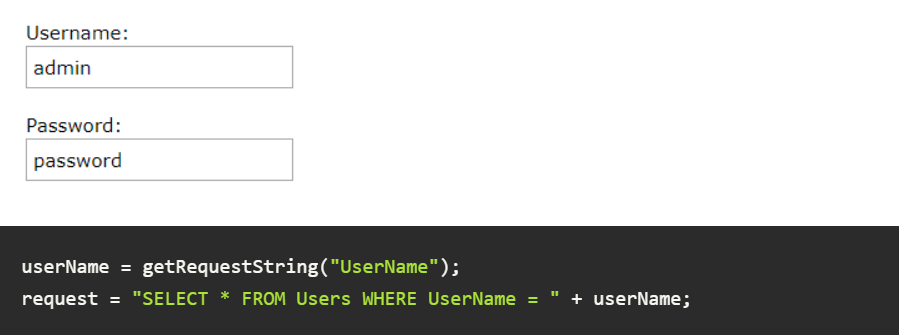
\includegraphics[width=0.8\textwidth]{assets/sql_ijection_example.png}
    \caption{Пример уязвимой страницы}
    \label{fig:mesh}
\end{figure}

\begin{itemize}
    \item \textbf{Атаки комментированием}\\
    Использование однострочных комментариев позволяет игнорировать часть запроса, идущую после вашей инъекции. Например, ввод в уязвимое поле Username запроса admin'-- позволит зайти на ресурс под администратором, потому что поверка пароля будет закомментирована.\\
    \begin{grayquote}
        SELECT * FROM members WHERE username = 'admin'--' AND password = 'password'
    \end{grayquote}

    Многострочные комментарии могут справится с проверкой или определить тип базы данных.
    Например, подобные запросы обойдут примитивный текстовый анализ:\\
    \begin{grayquote}
        DROP/*some comment*/sampletable\\
        DR/**/OP/*random comment to cheat*/sampletable
    \end{grayquote}

    \item \textbf{Манипуляции со строками}\\
    При помощи конкатенации строк можно обходить фильтр кавычек.\\
    \begin{grayquote}
        SELECT CONCAT(login, password) FROM members
    \end{grayquote}

    Можно представлять строки в шеснадцатиричном виде, с помощью функции HEX() или вводить их посимвольно.
    \begin{grayquote}
        //0x633A5C626F6F742E696E69 == c:\textbackslash boot.ini\\
        SELECT CONCAT('0x','633A5C626F6F742E696E69'))\\
        SELECT CONCAT(CHAR(75),CHAR(76),CHAR(77))
    \end{grayquote}

    \item \textbf{Обход аутентификации}\\
    При помощи OR и сравнения констант можно обойти форму аутентификации. Существуют даже словари, содержащие основные запросы для обхода уязвимой формы

    Примеры запросов:\\
    \begin{grayquote}
        ' or 1=1\\
        ' or 1=1--\\
        ' or 1=1\#\\
        admin' --\\
        admin' or '1'='1
    \end{grayquote}

    \item \textbf{Union injection}\\
    При помощи UNION комбинировать данные из разных таблиц в одну. Это одна из самых популярных и опасных классических инъекций.

    Допустим, на сайте есть список товаров с уязвимой строкой поиска. Тогда, подобрав правильное количество колонок и определив их название, через UNION можно вывести практически любые данные
    \begin{grayquote}
        SELECT name, price FROM products UNION ALL SELECT name, pass FROM members\\
        \#Такой запрос позволит получить данные о таблицах и найти таблицу пользователей\\
        UNION(SELECT TABLE\_NAME,

        TABLE\_SCHEMA FROM information\_schema.tables)
    \end{grayquote}

    \item \textbf{Расщепление SQL-запроса}\\
    В некоторых СУБД можно использовать простой знак ';' для последовательного вызова вредоносных запросов.
    
    Например, если в параметры скрипта
    \begin{grayquote}
    	\$id = \$\_REQUEST['id'];\\
    	\$res = mysql\_query("SELECT * FROM news WHERE id\_news = \$id");  
    \end{grayquote}
    злоумышленником передается конструкция, содержащая точку с запятой, например 12;INSERT INTO admin (username, password) VALUES ('HaCkEr', 'foo'); то в одном запросе будут выполнены 2 команды    	
    \begin{grayquote}
		SELECT * FROM news WHERE id\_news = 12;\\
   	 	INSERT INTO admin (username, password) VALUES ('HaCkEr', 'foo');
    \end{grayquote}
    и в таблицу admin будет несанкционированно добавлена запись HaCkEr.
    
    Также можно, к примеру, удалить таблицу или выключить SQL сервер.
    
    \begin{grayquote}
        \#Удаление таблицы\\
        SELECT * FROM products WHERE productName = ""; DROP users--\\
        \#Выключение SQL Server\\
        SELECT * FROM products WHERE productName = ""; shutdown –
    \end{grayquote}


    \item \textbf{Error-based injection}\\
    Инъекции, основанные на том, что злоумышленник может видеть вывод ошибки. Уязвимость устраняется просто отключением этого вывода

    Последовательное выполнение следующих запросов может помочь определить в тексте ошибки названия столбцов:\\
    \begin{grayquote}
        ' HAVING 1=1 --\\
        ' GROUP BY table.columnfromerror1 HAVING 1=1 --\\
        ' GROUP BY table.columnfromerror1, columnfromerror2 HAVING 1=1 --\\
        .....\\
        ' GROUP BY table.columnfromerror1, columnfromerror2, columnfromerror(n) HAVING 1=1 --\\
        Если ошибки перестали появляться, значит столбцы закончились
    \end{grayquote}

    \item \textbf{Boolean-based blind injection}\\
    Если атакующий все же может получить информацию о наличии или отсутствии ошибки из HTTP-статуса, в сервисе имеется уязвимость к обычной слепой атаке. Рассмотрим запрос, который позволит нам при помощи алгоритма бинарного поиска посимвольно определить название первой таблицы и в дальнейшем всех данных

    \begin{grayquote}
        TRUE : SELECT ID, Username, Email FROM [User]WHERE ID = 1 AND \\
        ISNULL(ASCII(SUBSTRING((SELECT TOP 1 name FROM sysObjects WHERE xtYpe=0x55 AND\\
        name NOT IN(SELECT TOP 0 name FROM sysObjects WHERE xtYpe=0x55)),1,1)),0)>78--\\
        \#Этот запрос говорит нам, что ASCII-значение первого символа больше 78 \\
        \#дальнейший перебор определит точное значение
    \end{grayquote}

    \item \textbf{Time-based blind injection}\\
    Если атакующий не наблюдает никаких отличий в ответах сервера, можно попробовать SLEEP или WAIT FOR DELAY

    \begin{grayquote}
        SELECT * FROM products WHERE id=1; WAIT FOR DELAY '00:00:15'
    \end{grayquote}
    Конечно, реальные примеры будут выглядеть примерно как boolean-based, только true и false атакующий будет отличать по времени отклика
    
        \item \textbf{Внедрение в строковые параметры}\\
   Предположим, серверное ПО, получив запрос на поиск данных в новостях параметром search\_text, использует его в следующем SQL-запросе (здесь параметры экранируются кавычками):\\
    \begin{grayquote}
    	\$search\_text = \$\_REQUEST['search\_text'];\\
    	\$res = mysqli\_query("SELECT id\_news, news\_date, news\_caption, news\_text, news\_id\_author\\
    	FROM news WHERE news\_caption LIKE('\%\$search\_text\%')");
    \end{grayquote}
    
    Сделав запрос вида http://example.org/script.php?search\_text=Test мы получим выполнение следующего SQL-запроса:\\
    \begin{grayquote}
    	SELECT id\_news, news\_date, news\_caption, news\_text, news\_id\_author FROM news 
    	WHERE news\_caption LIKE('\%Test\%')
    \end{grayquote}
    
        Но, внедрив в параметр search\_text символ кавычки (который используется в запросе), мы можем кардинально изменить поведение SQL-запроса. Например, передав в качестве параметра search\_text значение ')+and+(news\_id\_author='1, мы вызовем к выполнению запрос:\\
    \begin{grayquote}
    	SELECT id\_news, news\_date, news\_caption, news\_text, news\_id\_author FROM news 
    	WHERE news\_caption LIKE('\%') and (news\_id\_author='1\%')
    \end{grayquote}
    
    
\end{itemize}



\subsection{Экспертные ID-системы}

Название "экспертная система" происходит от термина "экспертная система, базирующаяся на знаниях". Экспертная система – это система, которая использует человеческие знания, встраиваемые в компьютер, для решения задач, которые обычно требуют человеческой экспертизы. Хорошо разработанные системы имитируют процесс рассуждения экспертов, используя это для решения специфических задач.

Технологию построения экспертных систем часто называют инженерией импликационных правил. Как правило,
этот процесс требует специфической формы взаимодействия создателя импликационных правил и одного
или нескольких экспертов в некоторой предметной области. Инженер импликационных правил "встраивает"
процедуры, стратегии, эмпирические правила в экспертную систему. В результате появляется
компьютерная программа, которая решает задачи во многом так же, как эксперты -- люди.
\autocite{IDSystem}

Главное преимущество использования продукционных систем заключается в возможности разделения причин и
решений возникающих проблем.

В экспертных системах могут использоваться импликационные правила (\textbf{Если} \textit{условие} то
\textbf{действие}).

Например:
\begin{itemize}
	\item ЕСЛИ с одного узла за время T поступает N пакетов, ТО записать в лог факт:
	происходит DoS атака (факт А)

	\item Если наблюдается более чем N фактов А, ТО записать в лог факт: происходит DDoS атака
\end{itemize}

Основные проблемы, которые обычно возникают при их практическом применении:
\begin{itemize}
    \item Недостаточная эффективность при работе с большими объемами данных.
    \item Трудно учесть зависимую природу данных параметров оценки.
\end{itemize}

При использовании экспертных систем для обнаружения вторжений можно установить символическое
проявление вторжения при помощи имеющихся данных.

\textbf{Трудности:}
\begin{itemize}
    \item Отсутствие встроенной или естественной обработки порядка последовательностей в анализируемых
    данных. База фактов, соответствующая левой части «продукции», используется для определения правой
    части. В левой части продукционного правила все элементы объединяются при помощи связи «и».
    \item Встроенная экспертиза хороша только в том случае, если моделируемые навыки администратора
    безопасности не противоречивы. Это практическое рассуждение, возможно, касается
    недостаточной централизованности усилий экспертов безопасности в направлении создания
    исчерпывающих множеств правил. Обнаруживаются только известные уязвимости.
    \item Существует определенный программный инжиниринг, связанный с установкой (поддержанием) баз знаний.
    При добавлении или удалении какого-либо из правил должно изменяться остальное множество правил.
    \item Обнаруживаются только известные уязвимости.
    \item Объединение различных измерений вторжений и создание связанной картины вторжения приводит к
    тому, что частные причины становятся неопределенными. Ограничения продукционных систем, в
    которых используется неопределенная причина, довольно хорошо известны.
\end{itemize}
\autocite{BeynonDavies}



\subsubsection{Метрики}

\begin{itemize}
	\item \textbf{Показатель активности} -- величина, при превышении которой активность
	подсистемы оценивается как быстро прогрессирующая. В общем случае используется для
	обнаружения аномалий, связанных с резким ускорением в работе. Пример: среднее число
	записей аудита, обрабатываемых для элемента защищаемой системы в единицу времени.

	\item \textbf{Распределение активности в записях аудита} -- распределение во всех типах
	активности в актуальных записях аудита. Здесь под активностью понимается любое действие
	в системе, например, доступ к файлам, операции ввода-вывода.

	\item \textbf{Измерение категорий} -- распределение определенной активности в
	категории \footnotemark. Например, относительная частота количества регистраций в
	системе (логинов) из каждого физического места нахождения. Предпочтения в использовании
	программного обеспечения системы (почтовые службы, компиляторы, командные интерпретаторы,
	редакторы и т.д.)

	\item \textbf{Порядковые измерения} -- используется для оценки активности, поступающей
	в виде цифровых значений. Например, количество операция ввода-вывода, инициируемых каждым
	пользователем. Порядковые изменения вычисляют общую числовую статистику значений определенной
	активности, в то время как измерение категорий подсчитывает количество активностей.
\end{itemize}
\autocite{BeynonDavies}
\footnotetext{Здесь под \textit{категорией} понимается группа подсистем, объединенных по
некоему общему принципу}



\subsubsection{Профили}

Используемые в настоящее время методы обнаружения аномалий основаны на общих представлениях теории распознавания образов. В соответствии с ними на основе экспертной оценки формируется \textbf{образ} нормального функционирования информационной системы. Этот образ выступает как совокупность значений параметров оценки. Отклонение от него считается проявлением аномального функционирования системы.

Один из способов формирования образа нормального поведения системы состоит в накоплении измерений значений параметров оценки в специальной структуре данных. Эта структура данных называется \textbf{профайлом} (профилем) \autocite{IDSystem}.

Основные требования, предъявляемые к структуре профайла:
\begin{itemize}
	\item Минимальный конечный размер

	\item Быстрое выполнение операции обновления
\end{itemize}



\subsubsection{Статистические модели для представления образа нормального поведения}

При обнаружении аномалий с использованием профайла в основном применяют статистические
методы оценки. Процесс обнаружения происходит следующим образом: текущие значения измерений
профайла сравнивают с сохраненными значениями. Результат сравнения - показатель аномальности
в измерении. Общий показатель аномальности в простейшем случае может вычисляться при помощи
некоторой общей функции от значений показателя аномалии в каждом измерении профайла.

Например, пусть $M_1, M_2, \dots, M_n$ -- измерения профайла, а $S_1, S_2, \dots, S_n$ --
соответственно представляют собой значения аномалии каждого из измерений. Чем больше
число $S_i$, тем больше аномалии в $i$-ом показателе. Объединяющая функция может быть
взвешенной суммой их квадратов:

\begin{equation}
	a_1s_1^2 + a_2s_2^2 + \dots + a_ns_n^2 > 0,
\end{equation}

где $a_i$ -- отражает относительный вес метрики $M_i$.

Параметры $M_1, M_2, \dots, M_n$ могут быть зависимыми друг от друга. В таком случае,
объединяющая функция будет более сложной.\autocite{IDSystem}

\textbf{Основное преимущество} заключается в том, что применяются хорошо известные статистические методы.

\textbf{Недостатки:}
\begin{itemize}
	\item Нечувствительность к последовательности возникновения событий.
	То есть статистическое обнаружение может упустить вторжение,
	которое проявляется в виде последовательности сходных событий.

	\item Система может быть последовательно обучена таким образом, что аномальное поведение
	будет считаться нормальным. Злоумышленники, которые знают, что за ними наблюдают
	при помощи таких систем, могут обучить их для использования в своих целях. Именно поэтому в
	большинстве существующих схем обнаружения вторжения используется комбинация подсистем
	обнаружения аномалий и злоупотреблений.

	\item Трудно определить порог, выше которого аномалии можно рассматривать как вторжение.
	Занижение порога приводит к ложному срабатыванию (false positive), а завышение – к пропуску вторжений (false negative).

	\item Существуют ограничения к типам поведения, которые могут быть смоделированы,
	используя чистые статистические методы. Применение статистических технологий для
	обнаружения аномалий требует предположения, что данные поступают от квазистатического процесса.
\end{itemize}
\autocite{IntrusionDetection}



\subsubsection{Нейронные сети для представления образа нормального поведения}
Другой способов представления "образа" нормального поведения системы – обучение нейронной
сети значениями параметров оценки.

Обучение нейронной сети осуществляется последовательностью информационных единиц (далее команд),
каждая из которых может находиться на более абстрактном уровне по сравнению с используемыми
параметрами оценки. Входные данные сети состоят из текущих команд и прошлых \textbf{W} команд, которые
обрабатываются нейронной сетью с целью предсказания последующих команд; \textbf{W} также называют размером
окна. После того как нейронная сеть обучена множеством последовательных команд защищаемой системы или
одной из ее подсистем, сеть представляет собой «образ» нормального поведения. Процесс обнаружения
аномалий представляет собой определение показателя неправильно предсказанных команд,
то есть фактически обнаруживается отличие в поведение объекта. На уровне рецептора стрелки
показывают входные данные последних \textbf{W} команд, выполненных пользователем. Входной параметр задает
несколько значений или уровней, каждый из которых уникально определяет команду. Выходной реагирующий
слой состоит из одного многоуровневого, который предсказывает следующую возможную команду пользователя.
\autocite{BeynonDavies}

\begin{figure}[h!]
    \centering
    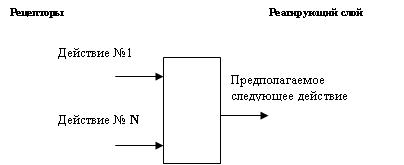
\includegraphics[width=0.8\textwidth]{assets/intrusion/neural_networks.jpg}
\end{figure}

\textbf{Недостатки:}
\begin{itemize}
    \item Топология сети и веса узлов определяются только после огромного числа проб и ошибок.
    \item Размер окна – еще одна величина, которая имеет огромное значение при разработке.
    Если сделать окно маленьким то сеть будет не достаточно производительной, слишком большим
    – будет страдать от неуместных данных.
\end{itemize}

\textbf{Преимущества:}
\begin{itemize}
    \item Успех данного подхода не зависит от природы исходных данных.
    \item Нейронные сети легко справляются с зашумленными данными.
    \item Автоматически учитываются связи между различными измерениями, которые,
    несомненно, влияют на результат оценки.
\end{itemize}
\autocite{BeynonDavies}


\subsubsection{Генерация паттернов для представления образа нормального поведения}
Представление «образа» в данном случае основывается на предположении о том, что текущие значения
параметров оценки можно связать с текущим состоянием системы. После этого функционирование
представляется в виде последовательности событий или состояний.

Были предложены временные правила, которые характеризуют совокупности значений параметров оценки
(далее паттерна) нормальной (не аномальной) работы. Эти правила формируются индуктивно и заменяются
более «хорошими» правилами динамически во время обучения. Под «хорошими правилами» понимаются правила
с большей вероятностью их появления и с большим уровнем уникальности для защищаемой системы.
Для примера рассмотрим следующее правило:

\begin{equation}
	E1 \rightarrow E2\rightarrow E3 \Rightarrow E4 = 0.95, E5 = 0.05
\end{equation}
где Е1\dotsЕ5 - события безопасности.

Это утверждение, основанное на ранее наблюдавшихся данных, говорит о том, что для последовательности
паттернов установилась следующая зависимость: если имеет место \textbf{Е1} и далее \textbf{Е2} и \textbf{Е3},
то после этого вероятность проявления \textbf{Е4} - 0.95 и \textbf{Е5} – 0.05.

Именно множество правил, создаваемых индуктивно во время наблюдения работы пользователя, составляет «образ».
Аномалия регистрируется в том случае, если наблюдаемая последовательность событий соответствует левой
части правила выведенного ранее, а события, которые имели место в системе после этого,
значительно отличаются от тех, которые должны были наступить по правилу.

\textbf{Основной недостаток} данного подхода заключается в том, что неузнаваемые паттерны поведения могут
быть не приняты за аномальные из-за того, что они не соответствуют ни одной из левых частей
всех правил.\autocite{IDSystem}

Данный метод довольно эффективно определяет вторжения, так как принимаются во внимание:
\begin{itemize}
    \item Зависимости между событиями.
    \item Последовательность появления событий.
\end{itemize}

\textbf{Достоинства метода:}
\begin{itemize}
    \item Лучшая обработка пользователей с большим колебанием поведения, но с четкой
    последовательностью паттернов.
    \item Возможность обратить внимание на некоторые важные события безопасности, а не на всю сессию,
    которая помечена как подозрительная.
    \item Лучшая чувствительность к обнаружению нарушений: правила содержат в себе семантику процессов, что позволяет гораздо проще заметить злоумышленников, которые пытаются обучить систему в своих целях.
\end{itemize}
\autocite{IntrusionDetection}

\subsubsection{Примеры ID-систем}


\paragraph*{GreenSQL} (APIDS система) -- межсетевой экран, функционирующий как
прокси-сервер между веб-приложением и SQL сервером. То есть приложение устанавливает
соединения к БД не напрямую, а через сервер GreenSQL. GreenSQL анализирует SQL запросы
на предмет аномальных запросов, и в случае нормального запроса (то есть если степень
риска запроса мала) перенаправляет его на внутренний сервер БД.

GreenSQL поддерживает следующие режимы работы:
\begin{itemize}
	\item \textbf{Режим симуляции (англ. Simulation Mode)} -- пассивная система обнаружения
	атак (IDS). Протоколирует SQL запросы, выдает предупреждения на консоль управления.

	\item \textbf{Блокировка подозрительных команд (англ. Blocking Suspicious Commands/Risk Based)} --
	активная СОВ. Атаки не только обнаруживаются, но и блокируются (IPS) в соответствии с
	установленными правилами, указывающими на аномальность запроса.

	\item \textbf{Активная защита от неизвестных запросов (англ. Database Firewall)} --
	блокирование всех неизвестных запросов.

	\item \textbf{Режим обучения (англ. Learning mode)} -- предназначен для прогона и
	настройки правил в <<чистой>> среде, что позволяет сформировать белый список и
	предотвратить в последствии ложные срабатывания анализатора запросов.
\end{itemize}

Особенности GreenSQL:
\begin{itemize}
	\item Поддержка ряда СУБД: Microsoft SQL 2000/2005/2008, MySQL 4.x/5.x, PostgreSQL 7.x/8.x.

	\item Является кросс-платформенной. Среди официально поддерживаемых платформ Microsoft
	Windows Server 2003/2008, Ubuntu, CentOS. Поддерживаются 32-х и 64-х разрядные системы.

	\item GreenSQL находит подозрительные запросы, используя ряд методов:
	\begin{itemize}
		\item Путем определения административных и чувствительных команд SQL.
		Например: SHOW TABLES, CREATE TABLE, ALTER TABLE.

		\item Путем подсчета риска запроса. На это может влиять пустая строка пароля, "or"
		внутри запроса или выражения SQL, которые всегда возвращают истину (1=1).
	\end{itemize}

\end{itemize}


\paragraph*{Snort} (NIDS система) -- свободная сетевая система предотвращения вторжений (IPS)
и обнаружения вторжений (IDS) с открытым исходным кодом, способная выполнять регистрацию
пакетов и в реальном времени осуществлять анализ трафика в IP-сетях.

Snort поддерживает следующие режимы работы:
\begin{itemize}
	\item \textbf{Sniffer mode}. В таком режиме программа только считывает сетевые пакеты и
	выводит их на консоль.

	\item \textbf{Packet Logger Mode}. В режиме логирования пакетов, программа будет
	регистрировать/логировать пакеты на диске.

	\item \textbf{Network Intrusion Detection System Mode}. В режиме обнаружения вторжений
	программа будет отслеживать сетевой трафик и анализировать его в соответствии с набором
	правил, определенным пользователем. Затем программа выполнит определенное действие,
	основанное на том, что было идентифицировано.
\end{itemize}

Особенности Snort:
\begin{itemize}
	\item Возможность написания собственных правил.
	\item Расширение функциональности с помощью подключения дополнительных модулей.
	\item Гибкая система оповещения об атаках: Log-файлы, устройства вывода, БД и прочие.
\end{itemize}


\paragraph*{Suricata} (NIDS система) -- свободная сетевая система предотвращения вторжений
(IPS) и обнаружения вторжений (IDS) с открытым исходным кодом. Основана разработчиками,
которые трудились над IPS версией Snort, поэтому имеет схожий функционал и обладает полной
поддержкой формата правил Snort.

Особенности Suricata:
\begin{itemize}
	\item Многозадачность.

	\item Автоматическое определение протокола.

	\item Высокая производительность, позволяющая обрабатывать трафик до 10Gbit на обычном
	оборудовании.
\end{itemize}


\paragraph*{Sagan} (HIDS система) -- многопоточная, высокопроизводительная система
анализа журналов и мониторинга появления в логах событий, связанных с безопасностью,
и реагирования на эти события в режиме реального времени. Система работает в операционных
системах Unix.

Sagan также относится к категории систем управления инцидентами и событиями информационной
безопасности (англ. Security Information and Log Management, SEIM).

\subsubsection{Недостатки существующих систем обнаружения}

Недостатки современных систем обнаружения можно разделить на две группы – недостатки, связанные со структурой СОВ, и недостатки, относящиеся к реализованным методам обнаружения.

\paragraph*{Недостатки структур СОВ.}

\begin{itemize}
	\item Отсутствие общей методологии построения. Частично это можно объяснить недостаточностью общих соглашений в терминологии, так как СОВ – это достаточно новое направление, основанное Андерсоном (J.P. Anderson) в 1980 г.
	\item Эффективность. Часто методы системы пытаются обнаружить любую понятную атаку, что приводит к ряду неудовлетворительных последствий. Например, при обнаружении аномалий существенно потребляется ресурсы – для любого профайла требуются обновления для каждого из наблюдаемых событий. При обнаружении злоупотреблений обычно используются командные интерпретаторы экспертных систем, при помощи которых кодируются сигнатуры. Очень часто эти командные интерпретаторы обрабатывают свое собственное множество правил и, соответственно, также потребляют ресурсы. Более того, множество правил разрешает только непрямые зависимости последовательности связей между событиями.
	\item Портативность. До сих пор большинство СОВ создается для использования на конкретном оборудовании, и достаточно трудно использовать их в другой системе, где требуется реализовать похожую политику безопасности. Например, задача по перемещению СОВ из системы, в которой поддерживается только одноуровневый список доступа, в систему с многоуровневой довольно сложна, и для ее решения потребуются значительные доработки. Основной причиной этого является то, что многие СОВ наблюдают за определенными устройствами, программами конкретной ОС. Также следует заметить, что каждая ОС разрабатывается для выполнения конкретных задач. Следовательно, переориентировать СОВ на другие ОС достаточно сложно, за исключение тех случаев, когда ОС разработаны в каком-то общем стиле.
	\item Возможности обновления. Очень сложно обновить существующие системы новыми технологиями обнаружения. Новая подсистема должна взаимодействовать со всей системой, и порой невозможно обеспечить универсальную возможность взаимодействия.
	\item Для установки СОВ очень часто требуются дополнительные навыки, существенно отличающиеся от навыков в области безопасности. Например, для обновления множества правил в системах обнаружения злоупотреблений требуются специализированные знания экспертной системы. Подобное можно сказать и про статические измерения системы обнаружения аномалий.
	\item Производительность и вспомогательные тесты – трудно оценить производительности СОВ в реальных условиях. Более того, отсутствует общий набор правил для тестирования СОВ, на основании которых можно было сказать о целесообразности использования данной системы в конкретных условиях и получить какие-то количественные показатели.
	\item Отсутствие хороших способов тестирования.
	
\end{itemize}

\paragraph*{Недостатки методов обнаружения:}

\begin{itemize}
	\item недопустимо высокий уровень ложных срабатываний и пропусков атак;
	\item слабые возможности по обнаружению новых атак;
	\item большинство вторжений невозможно определить на начальных этапах;
	\item трудно, иногда невозможно, определить атакующего, цели атаки;
	\item отсутствие оценок точности и адекватности результатов работы;
	\item невозможно определять «старые» атаки, использующие новые стратегии;
	\item сложность обнаружения вторжений в реальном времени с требуемой полнотой в высокоскоростных сетях;
	\item слабые возможности по автоматическому обнаружению сложных координированных атак;
	\item значительная перегрузка систем, в которых функционируют СОВ, при работе в реальном времени;
	
\end{itemize}



\subsubsection{Системы анализа и оценки уязвимостей}


Инструментальные средства анализа уязвимостей (известные также как оценка уязвимостей) тестируют сеть или хост для определения наличия уязвимостей для известных атак. Анализ уязвимостей предоставляет дополнительную информацию для систем обнаружения проникновения. Используемыми источниками информации являются атрибуты состояния системы и выходные данные осуществленных атак. Источники информации являются частью механизма оценки. Интервал времени анализа либо является фиксированным, либо определяется параметром в пакетном режиме, типом анализа является определение злоупотреблений. Это означает, что системы оценки уязвимостей являются пакетным режимом детекторов злоупотреблений, которые оперируют с информацией о состоянии системы, и результатом становятся специальные тестовые подпрограммы. \autocite{IntrusionDetectionSystemsMsu}

Анализ уязвимостей — очень сильная технология управления безопасностью, но эта технология является лишь дополнением к использованию IDS, а отнюдь не ее заменой. Если организация полагается исключительно на инструментальные средства анализа уязвимостей для слежения за системой, осведомленный атакующий может просмотреть систему анализа уязвимостей, заметить, когда выполняется анализ, и осуществить атаку во время интервала между этими проверками. 

Тем не менее системы анализа уязвимостей могут создавать ``моментальный снимок'' состояния безопасности системы в конкретное время. Более того, так как они являются исключительно тестовыми системами поиска уязвимостей для большого числа известных атак, системы анализа уязвимостей могут позволять менеджеру безопасности контролировать ошибки человека или выполнять аудит системы для анализа согласованности с конкретной политикой безопасности системы.

\paragraph*{Преимущества систем анализа уязвимостей:}

\begin{itemize}
	\item Анализ уязвимостей имеет важное значение как часть системы мониторинга безопасности, позволяя определять проблемы в системе, которые не может определить IDS.

	\item Системы анализа уязвимостей имеют возможность выполнять относящееся к безопасности тестирование, которое может использоваться для документирования состояния безопасности систем в момент начала функционирования программы безопасности или для переустановки базовых функций безопасности всякий раз, когда происходили существенные изменения.
	
	\item Когда системы анализа уязвимостей используются регулярно, они могут надежно обнаруживать изменения в состоянии безопасности системы, оповещая администраторов безопасности о проблемах, которые требуют решения.
\end{itemize}


\paragraph*{Недостатки и проблемы систем анализа уязвимостей:}

\begin{itemize}
	\item Некоторые network-based проверки, особенно касающиеся DoS-атак, могут разрушить систему, которую они тестируют.

	\item При выполнении оценки уязвимостей в сетях, в которых работают системы обнаружения проникновений, IDS могут блокировать проведение последующих оценок. Хуже того, регулярные network-based оценки могут ``обучить'' некоторые IDS, основанные на обнаружении аномалий, игнорировать реальные атаки.
\end{itemize}


\subsection{Системы управления событиями и информацией безопасности}

Системы управления событиями и информацией безопасности (англ. Security Information and Event Management / SIEM) представляют собой комплексное решение для мониторинга и анализа событий безопасности в реальном времени. Они собирают, обрабатывают и анализируют данные из различных источников, таких как сетевые устройства, серверы и приложения, чтобы выявлять и реагировать на угрозы \cite{SIEMSec}.

Основные свойства SIEM \cite{IBMSIEM}:
\begin{itemize}
    \item \textbf{Централизованный сбор данных}: SIEM агрегирует данные из множества источников, включая сетевые устройства, серверы, базы данных и приложения, что позволяет получить целостное представление о состоянии безопасности.
    \item \textbf{Корреляция событий}: Система анализирует данные, чтобы выявить взаимосвязанные события, которые могут указывать на сложные атаки. Это позволяет обнаруживать паттерны, которые могут остаться незамеченными при анализе отдельных событий.
    \item \textbf{Реальное время}: SIEM обеспечивает возможность мониторинга и реагирования на инциденты в реальном времени, что критично для минимизации ущерба от атак и быстрого восстановления нормальной работы.
\end{itemize}

Преимущества SIEM:
\begin{itemize}
    \item \textbf{Обширное покрытие}: SIEM позволяет мониторить различные компоненты IT-инфраструктуры, включая сетевые устройства, серверы и приложения, что обеспечивает комплексную защиту.
    \item \textbf{Ранняя детекция}: Система позволяет быстро выявлять инциденты безопасности, что уменьшает время реакции на угрозы и помогает предотвратить их распространение.
    \item \textbf{Комплексный анализ}: SIEM предоставляет углубленный анализ данных, что позволяет точно определить источник угроз и принять соответствующие меры.
\end{itemize}

Недостатки SIEM:
\begin{itemize}
    \item \textbf{Сложность внедрения}: Внедрение SIEM требует значительных ресурсов и времени на установку, настройку и интеграцию с существующими системами.
    \item \textbf{Высокая стоимость}: Затраты на приобретение, внедрение и обслуживание SIEM могут быть высокими, что делает их доступными не для всех организаций.
    \item \textbf{Ложные срабатывания}: Возможны ложные позитивные сигналы, которые требуют дополнительного анализа и могут отвлекать специалистов на несуществующие угрозы.
\end{itemize}


\subsection{Расширенное обнаружение и реагирование}

Расширенное обнаружение и реагирование (англ. eXtended Detection and Response / XDR) обеспечивает обнаружение инцидентов безопасности и возможности автоматического реагирования для инфраструктуры безопасности. XDR объединяет данные анализа угроз и телеметрии из различных источников с аналитикой безопасности для обеспечения контекстуализации и корреляции оповещений. XDR должен включать в себя встроенные датчики и может поставляться как в локальной сети, так и в виде SaaS-предложения. Как правило, его внедряют организации с небольшими командами безопасности.

Система работает за счет сбора и корреляции данных в различных точках сети, таких как серверы, электронная почта, облачные рабочие нагрузки и конечные устройства. Затем данные анализируются и коррелируются, придавая им видимость и контекст, а также выявляя современные угрозы. После этого угрозы приоритизируются, анализируются и сортируются, чтобы предотвратить крах системы безопасности и потерю данных. Система XDR помогает организациям повысить уровень кибернетической осведомленности, позволяя командам кибербезопасности выявлять и устранять уязвимости.

XDR улучшает возможности обнаружения вредоносных программ и антивирусов по сравнению с системой обнаружения и реагирования на конечные точки (англ. Endpoint Detection and Response / EDR). XDR совершенствует возможности EDR для развертывания высококлассных решений безопасности, используя современные технологии, которые проактивно выявляют и собирают угрозы безопасности, а также применяют стратегии для обнаружения будущих угроз кибербезопасности. Это альтернатива реактивным решениям для защиты конечных точек, таким как EDR и анализ сетевого трафика (англ. Network Traffic Analysis / NTA).

Сейчас, когда мы немного разобрались со структурой XDR, предлагаю обсудить, как на текущий момент выглядит информационная безопасность в компаниях. Приведу пример.

У компании есть агенты антивирусной защиты на конечных станциях, есть свой прокси сервер, антиспам. Получается достаточно классический набор СЗИ. Данные СЗИ фактически никаким образом между собой не связаны, и вполне логичным будет поставить дополнительно систему управления событиями информационной безопасности (SIEM). Теперь все события объединены в одном месте, но никакой интеграции между этими системами все равно нет, и автоматизации, как вы понимаете – тоже. Конечно, для реагирования на инциденты ИБ можно внедрить еще одну дополнительную систему – SOAR (англ. Security Orchestration, Automation and Response). И вот мы уже получили достаточно большой и сложный в эксплуатации комплекс СЗИ по информационной безопасности.

Может ли XDR как-то помочь упростить процесс расследования и реагирования на инциденты? – Да, может.

В случае использования XDR, при обнаружении угрозы в любом из источников трафика, появляется возможность в полуавтоматическом режиме (без написания специальных сценариев реагирования - плейбуков) осуществлять блокирование данной угрозы, в том числе и с помощью агентов на рабочих станциях пользователей, что невозможно в классической модели, описанной выше. Также, в отличие от SOAR, в XDR для реагирования уже подготовлены специальные наборы команд, которые можно запускать прямо из веб-интерфейса, например, изоляция станций, удаление файлов и др.

Выше я привел лишь один из примеров, показывающих актуальность XDR. Если попробовать достаточно обобщенно выделить все ключевые преимущества, которые получает компания при построении концепции XDR, то получится следующий результат:

\begin{itemize}

\item Контроль всех наиболее популярных точек входа злоумышленников в IT-инфраструктуру

\item Обнаружение цепочек атак

\item Централизованная обработка событий ИБ со всех компонентов XDR

\item Расширенный анализ событий с конечных устройств, за счет чего удается обнаруживать скрытые от обычных антивирусов угрозы

\item Наличие инструментов по оперативному реагированию на угрозы (изоляция станций, удаление файлов, поиск индикаторов компрометации, завершение процессов, запуск скриптов, получение дампов памяти и др.)

\item Сокращение времени на расследование инцидентов

\item Динамические методы анализа (Sandbox) – поиск угроз нулевого дня, на всех уровнях инфраструктуры

\item Обогащение данных за счет интеграции с платформой Threat Intelligance

\item Интеграция со сторонними системами защиты
\end{itemize}


\subsection{Индикаторы компрометации}

Индикаторы компрометации (англ. Indicator of Compromise / IOC) представляют собой артефакты, такие как файлы, хэши, IP-адреса, которые указывают на то, что система была скомпрометирована. IOC используются для идентификации и реагирования на инциденты безопасности.

Основные свойства IOC:
\begin{itemize}
    \item \textbf{Идентификация угроз}: IOC позволяют определить специфические артефакты, которые связаны с определёнными типами угроз. Это могут быть хэши файлов, IP-адреса, домены, связанные с вредоносной активностью.
    \item \textbf{Автоматизация}: Возможность автоматического применения индикаторов для выявления угроз позволяет значительно ускорить процесс обнаружения и реакции на инциденты.
    \item \textbf{Обмен информацией}: Обмен IOC между организациями способствует коллективной безопасности, позволяя быстрее реагировать на новые угрозы и делиться актуальной информацией.
\end{itemize}

Преимущества IOC:
\begin{itemize}
    \item \textbf{Быстрое реагирование}: Использование IOC позволяет оперативно обнаруживать и реагировать на инциденты, минимизируя возможный ущерб.
    \item \textbf{Точность}: Высокая точность при идентификации известных угроз, что позволяет эффективно защищать системы от повторных атак.
    \item \textbf{Совместимость}: Возможность интеграции с различными системами безопасности и автоматизации процессов обнаружения угроз.
\end{itemize}

Недостатки IOC:
\begin{itemize}
    \item \textbf{Ограниченность}: IOC эффективны только для выявления известных угроз и могут быть бесполезны против новых, ранее неизвестных атак.
    \item \textbf{Требуют обновлений}: Необходимость регулярного обновления базы данных индикаторов для поддержания их актуальности и эффективности.
    \item \textbf{Зависимость от источников}: Эффективность IOC сильно зависит от качества и актуальности предоставленных индикаторов, что требует надежных источников информации (Неговора и др., 2020).
\end{itemize}

\subsection{Примеры современных IDS и SIEM}

В этом разделе рассмотрим пять современных примеров IDS и SIEM, выделив их особенности и предоставив ссылки для получения дополнительной информации.

\subsubsection{Splunk}

Splunk — это мощная платформа для анализа данных, которая также включает функции SIEM. Она собирает и анализирует данные из различных источников, включая журналы событий, сетевой трафик и данные приложений.

Особенности Splunk:
\begin{itemize}
    \item \textbf{Масштабируемость}: Поддержка больших объемов данных и масштабирование по мере роста потребностей.
    \item \textbf{Реальное время}: Анализ данных и обнаружение угроз в реальном времени.
    \item \textbf{Интеграция}: Широкие возможности интеграции с другими инструментами безопасности.

\end{itemize}

Дополнительная информация доступна по ссылке: \url{https://www.splunk.com/}

\subsubsection{AlienVault OSSIM}

AlienVault OSSIM (Open Source SIEM) — это популярная платформа с открытым исходным кодом для управления событиями безопасности. Она объединяет возможности IDS, SIEM и управления уязвимостями.

Особенности AlienVault OSSIM:
\begin{itemize}
    \item \textbf{Комплексность}: Объединение различных инструментов безопасности в одну платформу.
    \item \textbf{Открытый исходный код}: Возможность модификации и адаптации под специфические нужды.
    \item \textbf{Обширная база данных угроз}: Использование данных из многочисленных источников для улучшения обнаружения угроз.
\end{itemize}

Дополнительная информация доступна по ссылке: \url{https://cybersecurity.att.com/products/ossim}

\subsubsection{Snort}

Snort — это популярная система обнаружения вторжений с открытым исходным кодом, разработанная для анализа сетевого трафика в режиме реального времени. Она может работать как IDS или как инструмент предотвращения вторжений (IPS).

Особенности Snort:
\begin{itemize}
    \item \textbf{Гибкость}: Возможность настройки под конкретные нужды пользователя.
    \item \textbf{Сообщество пользователей}: Поддержка активного сообщества и регулярные обновления.
    \item \textbf{Масштабируемость}: Возможность использования в различных масштабах, от небольших сетей до крупных корпоративных систем.
\end{itemize}

Дополнительная информация доступна по ссылке: \url{https://www.snort.org/}

\subsubsection{IBM QRadar}

IBM QRadar — это мощная SIEM-платформа, предназначенная для мониторинга, анализа и реагирования на инциденты безопасности. Она собирает данные из различных источников и использует передовые методы аналитики для обнаружения угроз.

Особенности IBM QRadar:
\begin{itemize}
    \item \textbf{Машинное обучение}: Использование методов машинного обучения для улучшения точности обнаружения угроз.
    \item \textbf{Интеграция}: Широкие возможности интеграции с другими системами и инструментами безопасности.
    \item \textbf{Реальное время}: Обнаружение и реагирование на инциденты в реальном времени.
\end{itemize}

Дополнительная информация доступна по ссылке: \url{https://www.ibm.com/security/security-intelligence/qradar}

\subsubsection{Palo Alto Networks Cortex XDR}

Palo Alto Networks Cortex XDR — это платформа для обнаружения и реагирования на угрозы, которая объединяет возможности IDS и SIEM. Она предоставляет комплексный подход к безопасности, объединяя данные из различных источников для улучшения анализа и реагирования.

Особенности Cortex XDR:
\begin{itemize}
    \item \textbf{Единая платформа}: Объединение данных и аналитики для всестороннего анализа угроз.
    \item \textbf{Машинное обучение}: Использование передовых алгоритмов для улучшения точности обнаружения.
    \item \textbf{Автоматизация}: Автоматизация процессов обнаружения и реагирования на угрозы.
\end{itemize}

Дополнительная информация доступна по ссылке: \url{https://www.paloaltonetworks.com/cortex/xdr}


\subsection{Развитие систем распознавания вторжений}

\subsubsection{Развитие практических аспектов СОВ}

Коммерческое использование СОВ находится в стадии формирования. Некоторые коммерческие
СОВ получили негативную публичную оценку за большое число ложных срабатываний, неудобные
интерфейсы управления и получения отчетов, огромное количество отчетов об атаках,
плохое масштабирование и плохую интеграцию с системами сетевого управления. Тем не менее
потребность в хороших СОВ возрастает, поэтому с большой вероятностью эти проблемы будут
успешно решаться в ближайшее время.

Ожидается, что улучшение качества функционирования СОВ будет осуществляться аналогично
антивирусному ПО. Раннее антивирусное ПО создавало большое число ложных тревог при
нормальных действиях пользователя и не определяло все известные вирусы. Однако сейчас
положение существенно улучшилось, антивирусное ПО стало прозрачным для пользователей
и достаточно эффективным.

Более того – очень вероятно, что основные возможности СОВ скоро станут ключевыми в
сетевой инфраструктуре (такой как роутеры, мосты и коммутаторы) и в операционных системах.
При этом, скорее всего, разработчики СОВ сфокусируют свое внимание на решении проблем,
связанных с масштабируемостью и управляемостью СОВ.

Имеются также и другие тенденции, которые, скорее всего, будут влиять на функциональности
СОВ следующего поколения. Существует заметное движение в сторону аппаратно-программных
(appliance) решений для СОВ. Также вероятно, что в будущем некоторые функции определения
соответствия шаблону могут быть реализованы в аппаратуре, что увеличит скорость обработки.

Наконец, механизмы, связанные с управлением рисками в области сетевой безопасности,
будут оказывать влияние на требования к СОВ.



\subsubsection{Развитие теоретических аспектов СОВ}

Дальнейшие направления совершенствования связаны с внедрением в теорию и практику СОВ
общей теории систем, методов синтеза и анализа информационных систем, конкретного аппарата
теории распознавания образов. Эти разделы теории предполагают получение конкретных методов
исследования для области систем СОВ.

До настоящего времени не описана СОВ как подсистема информационной системы в терминах
общей теории систем. Необходимо обосновать показатель качества СОВ, элементный состав
СОВ, ее структуру и взаимосвязи с информационной системой.

В связи с наличием значительного количества факторов различной природы, слаженная работа
информационной системы и СОВ имеет вероятностный характер. Вследствие этого актуальным
является обоснование вида вероятностных законов конкретных параметров функционирования.
Особо следует выделить задачу обоснования функции потерь информационной системы, задаваемую
в соответствии с ее целевой функцией на области параметров функционирования системы.
При этом целевая функция должна быть определена не только на экспертном уровне, но и в
соответствии с совокупностью параметров функционирования всей информационной системы и
задачами, возложенными на нее. В таком случае показатель качества СОВ будет определяться
как один из параметров, влияющих на целевую функцию, а его допустимые значения --
допустимыми значениями функции потерь.

После обоснования законов и функций, реальной задачей является получение оптимальной
структуры СОВ в виде совокупности математических операций с помощью формализованных
методов. Таким образом, может быть решена задача синтеза структуры СОВ. На основе
полученных математических операций можно будет рассчитать зависимости показателей
качества функционирования СОВ от параметров ее функционирования, а также от параметров
функционирования информационной системы, то есть, будет возможен реальный анализ качества
функционирования СОВ.

Сложность применения формализованного аппарата анализа и синтеза информационных систем
к СОВ заключается в том, что конкретные реализации информационного комплекса и его
подсистемы - СОВ состоят из разнородных элементов, которые могут описываться различными
разделами теории (системами массового обслуживания, конечными автоматами, теорией
вероятности, теорией распознавания образов и т.д.), то есть, рассматриваемый объект
исследования является составным. В результате, математические модели, по-видимому,
можно получить только для отдельных составных частей СОВ, что затрудняет анализ и
синтез СОВ в целом. Однако, дальнейшая конкретизация применения формализованного
аппарата анализа и синтеза позволит оптимизировать СОВ.

На основе изложенного можно сделать вывод о наличии в практической среде значительного опыта
решения проблем обнаружения вторжений. Применяемые СОВ в значительной степени основаны на
эмпирических схемах процесса обнаружения вторжений. Дальнейшее совершенствование СОВ связано
с конкретизацией методов синтеза и анализа сложных систем, теории распознавания образов в
применении к СОВ.
